\authoredSection{julius}{User-Interface \& User-Experience}

\subsection{Mockups}
	Vor Beginn der Gestaltung der Mockups haben wir uns auf dem Markt der Banking-Apps umgeschaut, um die verschiedenen UI-Patterns, die in diesem Zusammenhang genutzt werden, zu vergleichen. Mit Balsamiq entwarfen wir anschließend erste Mockups. Bei der Anordnung der Elemente haben wir uns die Prinzipien der Gestaltungsgesetze zunutze gemacht. Insbesondere halfen uns das Gesetz der Ähnlichkeit und das Gesetz der Nähe, Ordnung in die UI zu bringen. 

	Unser Ziel war es, ein möglichst gebrauchstaugliches Design zu erreichen. Dazu haben wir uns an den Grundsätzen der Dialoggestaltung nach der DIN EN ISO 9241 110 orientiert. Bei der Gestaltung haben wir nur eine Schriftart verwendet und uns nach festgelegte Farbsemantiken gerichtet. Dadurch geht der Fokus auf den Inhalt nicht verloren und der Nutzer kann die App erwartungskonform nutzen. Bei der Navigation haben wir uns für eine Master-Detail-View entschieden. Dadurch haben wir eine flache Navigationshierarchie, die es uns ermöglicht, alle wichtigen Funktionen von der Hauptseite direkt zu erreichen. Auf diese Weise haben wir unnötige Interaktionen minimiert und der Nutzer kann effizient und aufgabenangemessen mit der App interagieren.  

	Auf jeder Detail-View befindet sich unten rechts ein Informationbutton. Mit diesem Button wollen wir die Selbstbeschreibungsfähigkeit der App verbessern und die Nutzer bei Problemen unterstützen.
	
\begin{figure}[p]
	\centering
	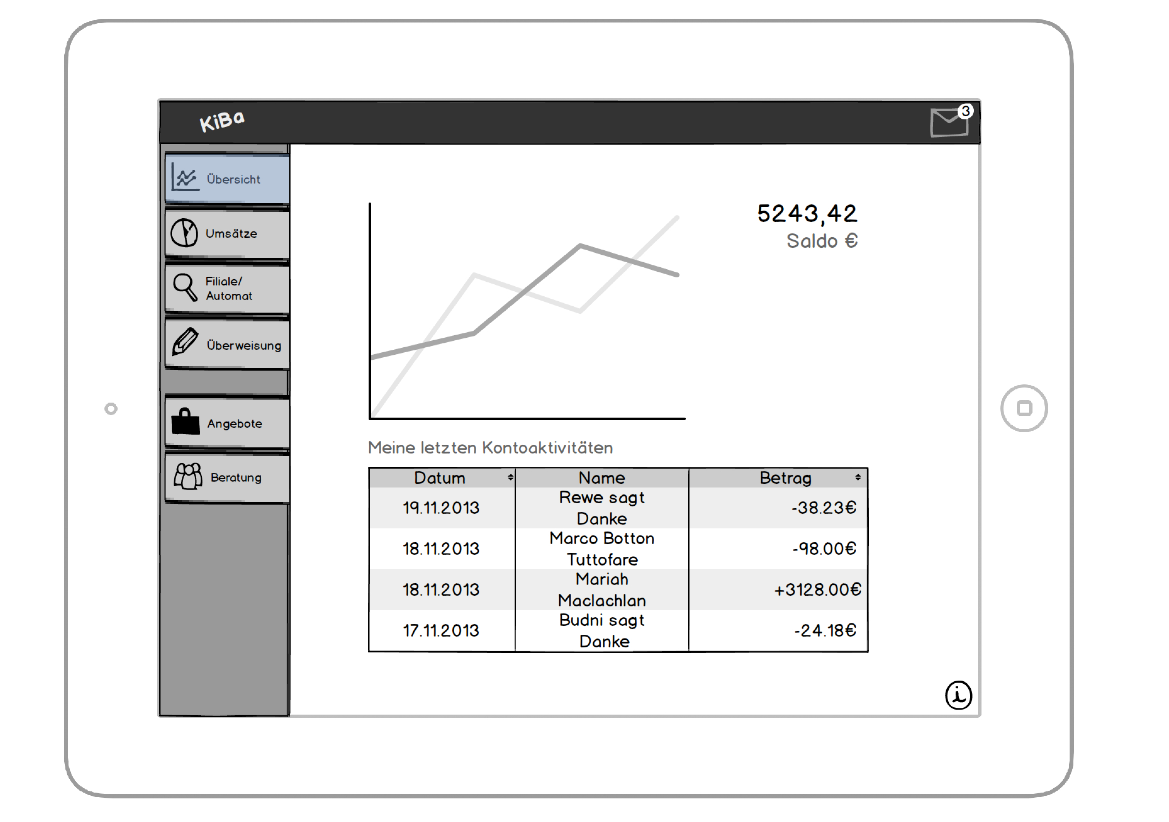
\includegraphics[scale=.52]{Pictures/MockupDashboard}\\
	\includegraphics[scale=.52]{Pictures/MockupBranch}\\
	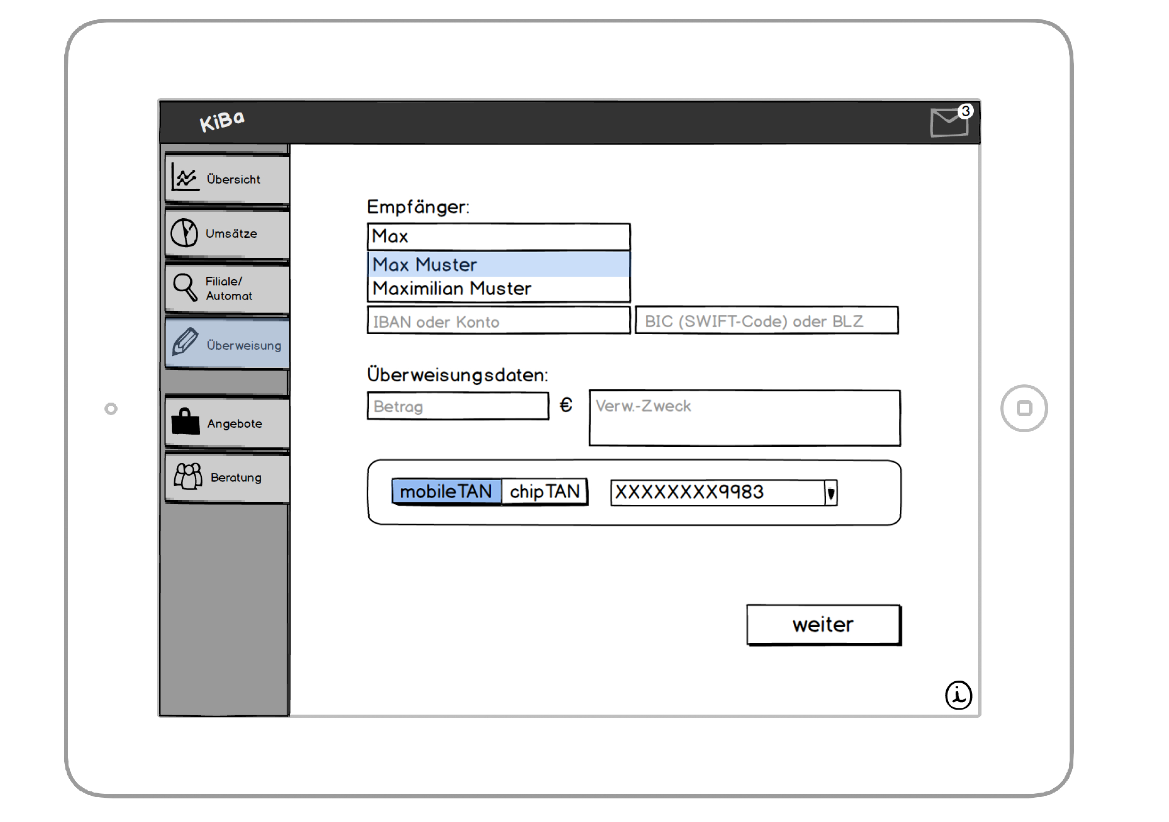
\includegraphics[scale=.52]{Pictures/MockupTransition}
	\caption{Mockup des Dashboards, der Filial-Seite und der Überweisung}
\end{figure}

	Die Elemente in der Detail-View sind asymmetrisch angeordet mit einer Gewichtung oben links und unten rechts. So erreichen wir eine diagonale Balance, die optimal für den optischen Fluss ist.

\subsection{Prototyp}
	Allgemein haben wir uns beim Design des User-Interface an den Guidelines von IOS7 orientiert. In diesem Zusammenhang haben wir uns mit den wichtigsten Grundsätzen laut Apple „Deference“, „Clarity“ und „Depth“ beschäftigt, um diese auf unser User-Interface zu übertragen. 
	
	„Deference“ haben wir bewirkt, indem wir den Fokus auf die Wahrnehmung von Inhalten gelegt haben und versucht haben, UI-Elemente, die in Konflikt mit dem Inhalt stehen, wegzulassen. Uns war es wichtig, das User-Interface möglichst funktional zu gestalten, was auch im Sinne von „Clarity“ ist. Daher haben wir eine möglichst selbsterklärende Ikonographie gewählt und auf eine unnötige Farbenvielfalt verzichtet. Den Guidelines entsprechend haben wir die Icons mindestens in der Größe 44 $\times$ 44 pts dimensioniert. Andernfalls wird es schwierig, ein Icon mit dem Finger zu treffen. Außerdem gibt es zu jedem Icon 2 Versionen, damit auf einem Retina iPad die hohe Auflösung ausgenutzt werden kann. Mit iOS7 setzt Apple auf Flat-Design. Ganz im Sinne des Flat-Designs haben wir mit kräftigen Kontrasten statt mit Schlagschatten oder Gradienten gearbeitet. Darüber hinaus wurde eine dünne, serifenlose Schriftart gewählt.

	Aufgrund von leichten Konzeptänderungen während des Projekts haben wir manche Details im Prototypen anders als in den Mockups gestaltet.
	
	Beispielsweise gab uns Markus Foos den Tipp, dass Nutzer mehr interessiert sind an den Umsätzen als an dem aktuellen Kontostand. Das ist besonders der Fall bei denjenigen Leuten, deren Kontostand niedrig ist oder die sogar im Minus liegen. \par

\begin{figure}[h]
	\centering
	
\includegraphics[scale=.52]{Pictures/Logo}
	\caption{App-Icon mit Farbskala}
\end{figure}
\subsection{Logo \& Farbharmonie}
	Unsere ausgewählte Farbharmonie spiegelt die Werte einer modernen Bank wider. Mit den Farben wollen wir Sicherheit, Nachhaltigkeit und Seriosität vermitteln. Allerdings waren wir bei der Logogestaltung in dieser Hinsicht nicht ganz konsequent. Wir hatten an dieser Stelle die Diskussion, ob wir uns nicht für ein anderes Logo entscheiden sollten. Mit dem KiBa-Glas im Logo haben wir uns dann darauf geeinigt, als Studenten ein wenig Humor zuzulassen. Im Zusammenspiel mit dem recht nüchternen Design wirkt das Logo auflockernd.

\subsection{UI-Elemete}
	Grundsätzlich haben wir mit den Standard-View-Elementen von iOS7 gearbeitet. Allerdings haben wir in machen Fällen auf ein Custom-Element zurückgegriffen und dieses dann konsequent eingesetzt. Bei dem Standard-Text-Field störte uns etwa, dass der Hint-Text bei der Eingabe verschwand und so die Eingabe gelöscht werden musste, um diesen wieder zu sehen. Man stelle sich vor, man möchte ein Überweisungsformular ausfüllen und während der Eingabe eines Feldes ist man sich nicht mehr sicher, wofür dieses steht. 

	Daher entschieden wir uns für eine Eigenlösung, die den Vorteil hat, dass der Hint-Text bei erfolgter Eingabe nach oben rückt und auf diese Weise sichtbar bleibt. 

\subsection{UX Inspektion \& Test}
	Wöchentlich hatten wir im Plenum die Möglichkeit, unseren Stand der App vorzustellen. Hier konnten in einer anschließenden Diskussion Unklarheiten im Konzept und Design angesprochen werden. Da sich im Plenum unter anderem Dr. Kindsmüller befand, konnten wir von dem Wissen eines erfahrenen UX-Experten profitieren. Beispielsweise deckte er auf, dass wir eine Geste nicht erwartungskonform verwendeten. Bei der Scheck-Überweisung wollten wir anfangs mit der Wischgeste nach unten die Überweisung abschicken. Allerdings wird diese Wischgeste normalerweise als „Pull-to-refresh“-Geste verwendet. Daher war hier die Affordanz (Angebotscharakter) nicht gegeben. Um Verwirrung beim potentiellen Nutzer zu vermeiden, haben wir die Geste durch einen einfachen Button zum Abschicken der Überweisung ersetzt und die Animation entsprechend angepasst.

	Zwischendurch haben wir auch Kommilitonen die KiBa-App testen lassen. Wir stellten bei diesen kleinen Usability-Tests fest, dass das Konzept und der Sinn hinter der Authentifizierung nicht ganz verständlich war. Daher entschieden wir uns einen Comic zu erstellen, der die Kernschritte und Vorteile explizit erklärt. Auch ging aus der App nicht hervor, bei welchen Funktionen die Authentifizierung eine Rolle spielt. Diesen Mangel behoben wir, indem wir die Funktionen, welche erst nach der Authentifizierung verwendbar sind, mit einem Schloss-Icon markierten.
	
	Im Schlusssprint hatten wir die Möglichkeit, mit Herrn Kindsmüller jede View zu inspizieren, um auch die kleinen Interaktionsmängel aufzudecken. Beim Comic, der das Authentifizierungsverfahren erklärt, war beispielsweise der „Vorteil genießen“- Button für Nutzer nicht auffordernd genug. Dieses Problem der Salienz lösten wir durch eine leichte Animation. Des Weiteren wurde bei dem Kreditrechner nicht klar, dass individuelle Konditionen beim Berechnen eine Rolle spielen. Hier wurde uns vorgeschlagen, persönliche Assoziationen zu verwenden, wie „Ihr  Kreditrechner“ oder „Johns Kreditrechner“.

	All diese Erfahrungen zeigten uns, wie wichtig es ist, Kritik von außen einzuholen. Da wir in der Gruppe viel Vorwissen hatten, erschienen uns Dinge eindeutig, die für spätere Nutzer nicht unbedingt eindeutig sind.
Sicherlich wäre besser gewesen, früher mit dem Testen anzufangen.

	Dadurch das wir mit High-Fidelity-Prototypen getestet haben, gab es hauptsächlich Feedback zu kleineren Details und das gesamte Konzept wurde nicht in Frage gestellt. Trotzdem haben wir viel hilfreiche Kritik bekommen und konnten auf diese Weise mögliche Abbruchstellen in der UI beseitigen.
